\documentclass{article}

\usepackage{fancyhdr}
\usepackage{extramarks}
\usepackage{amsmath,esint}
\usepackage{amssymb}
\usepackage{amsthm}
\usepackage{amsfonts}
\usepackage{tikz}
\usepackage[plain]{algorithm}
\usepackage{algpseudocode}
\usepackage{enumitem}
\usepackage{mathtools}
\usepackage{siunitx}
\graphicspath{ {./images/}}

\usetikzlibrary{automata,positioning}

\newcommand*\VF[1]{\mathbf{#1}}
\newcommand*\dif{\mathop{}\!\mathrm{d}}


%
% Basic Document Settings
%

\topmargin=-0.45in
\evensidemargin=0in
\oddsidemargin=0in
\textwidth=6.5in
\textheight=9.0in
\headsep=0.25in

\linespread{1.1}

\pagestyle{fancy}
\lhead{\hmwkAuthorName}
\chead{Study Guide For 33-142 Summer 2018}
\rhead{Professor Ghosh}
\lfoot{\lastxmark}
\cfoot{\thepage}

\renewcommand\headrulewidth{0.4pt}
\renewcommand\footrulewidth{0.4pt}

\setlength\parindent{0pt}

%
% Create Problem Sections
%

\newcommand{\enterProblemHeader}[1]{
    \nobreak\extramarks{}{Problem \arabic{#1} continued on next page\ldots}\nobreak{}
    \nobreak\extramarks{Problem \arabic{#1} (continued)}{Problem \arabic{#1} continued on next page\ldots}\nobreak{}
}

\newcommand{\exitProblemHeader}[1]{
    \nobreak\extramarks{Problem \arabic{#1} (continued)}{Problem \arabic{#1} continued on next page\ldots}\nobreak{}
    \stepcounter{#1}
    \nobreak\extramarks{Problem \arabic{#1}}{}\nobreak{}
}

\setcounter{secnumdepth}{0}
\newcounter{partCounter}
\newcounter{homeworkProblemCounter}
\setcounter{homeworkProblemCounter}{1}
\nobreak\extramarks{Problem \arabic{homeworkProblemCounter}}{}\nobreak{}

%
% Homework Problem Environment
%
% This environment takes an optional argument. When given, it will adjust the
% problem counter. This is useful for when the problems given for your
% assignment aren't sequential. See the last 3 problems of this template for an
% example.
%
\newenvironment{homeworkProblem}[1][-1]{
    \ifnum#1>0
        \setcounter{homeworkProblemCounter}{#1}
    \fi
    \section{Problem \arabic{homeworkProblemCounter}}
    \setcounter{partCounter}{1}
    \enterProblemHeader{homeworkProblemCounter}
}{
    \exitProblemHeader{homeworkProblemCounter}
}

%
% Homework Details
%   - Title
%   - Due date
%   - Class
%   - Section/Time
%   - Instructor
%   - Author
%

\newcommand{\hmwkTitle}{Homework\ \#11}
\newcommand{\hmwkDueDate}{May 1, 2018}
\newcommand{\hmwkClass}{21-127 Concepts}
\newcommand{\hmwkClassTime}{Section A}
\newcommand{\hmwkClassInstructor}{Professor Ghosh}
\newcommand{\hmwkAuthorName}{\textbf{William Cen}}
\newcommand{\eqn}{\[
    \stcomp{(A \cup B)} = \stcomp{A} \cap \stcomp{B}
\]}

%
% Title Page
%

\title{
    \vspace{2in}
    \textmd{\textbf{Study Guide For 33-142 Physics 2}}\\
    %\normalsize\vspace{0.1in}\small{Due\ on\ \hmwkDueDate\ at 3:10pm}\\
    \vspace{0.1in}\large{\textit{\hmwkClassInstructor}}
    \vspace{3in}
}

\author{\hmwkAuthorName}
\date{}

\renewcommand{\part}[1]{\textbf{\large Part \Alph{partCounter}}\stepcounter{partCounter}\\}

%
% Various Helper Commands
%

% Useful for algorithms
\newcommand{\alg}[1]{\textsc{\bfseries \footnotesize #1}}

% For derivatives
\newcommand{\deriv}[1]{\frac{\mathrm{d}}{\mathrm{d}x} (#1)}

% For partial derivatives
\newcommand{\pderiv}[2]{\frac{\partial}{\partial #1} (#2)}

% Integral dx
\newcommand{\dx}{\mathrm{d}x}

% Alias for the Solution section header
\newcommand{\solution}{\textbf{\large Solution}}

% Probability commands: Expectation, Variance, Covariance, Bias
\newcommand{\E}{\mathrm{E}}
\newcommand{\Var}{\mathrm{Var}}
\newcommand{\Cov}{\mathrm{Cov}}
\newcommand{\Bias}{\mathrm{Bias}}

\begin{document}

\maketitle

\pagebreak
\section{General Knowledge}
What you should know:\\
\label{definitions}
\begin{description}
\item[Vectors]
Example: $\vec{E} = \frac{q}{4\pi\epsilon |r|^3}\vec{r}$\\
An abstract tool useful for physics. It has a direction and magnitude, so you can use vectors to describe anything that depends on direction, such as electric fields. 

\item[Unit Vectors]
Example: $\hat{r} = \frac{\vec{r}}{|\vec{r}|}$\\
A vector with magnitude 1. This is quite important when describing direction. In fact, our definition of the electric field above can be condensed to: $\vec{E} = \frac{q}{4\pi\epsilon r^2} \hat{r}$

\item[The "r" vector]
Just a vector describing radial direction. Conveniently, this is also $\vec{r} = r <cos(\theta), sin(\theta)>$

\item[Coulomb (C)]
SI unit of measurement for charge

\item[$\epsilon$]
Constant of dielectric permitivity. Larger epsilons lead to... You'll find out later in class :)

\end{description} 

\subsection{Useful Constants}
$Q_{\text{proton/electron}} = \pm1.60 * 10^{-19} \text{C}$\\
\\
$\frac{1}{4\pi\epsilon_0} = 8.99 * 10^9 N\cdot m^2 \cdot C^{-2}$ Note that $\epsilon_0$ is used here because this refers to the constant of dielectric permitivity in a vacuum (which we will frequently use) \\
\\
$\hat{i}, \hat{j}, \hat{k} = $ x, y, z unit vectors: $<1,0,0>, <0,1,0>, <0,0,1>$
\subsection{Important Concepts}
\textbf{Coulomb's Law}: $\vec{F}_{\text{Coulomb}} = \frac{1}{4\pi\epsilon} \frac{Q_1 Q_2}{|r|^2} \hat{r}$\\
\\
\textbf{Superposition Principle}: A principle that describes that the net effect at a point in space is the net sum of all the individual effects from all sources at that point. This can be simplified to our description of electric fields. The net electric field at a point is the sum of all individual electric fields at that point: $\vec{E}_{net} = \Sigma \vec{E}_i$.\\
\\
\textbf{Conservative System}: In a conservative system, all energy is conserved. This also means that there are no external forces involved, since the source and effect is all contained within the system. For example, a system that has 2 charges and only has the fields due to those two charges is conservative. However, if you enclose the effects of both but only one of those charges, then the electric field due to the charge not in your system is an "external" effect.\\

\subsection{Useful Equations}
\textbf{Dot Product}: Say $\vec{u} = <u_x, u_y>, \vec{v} = <v_x, v_y>$, then  $\vec{u} \cdot \vec{v} = u_x*v_x + u_y*v_y = |\vec{u}||\vec{v}|cos(\theta)$ \\
\\
\textbf{Cross Product}: Say $\vec{u} = <u_x, u_y, u_z>, \vec{v} = <v_x, v_y, u_z>$, then 

\[
\vec{u} \times \vec{v} =
    \begin{vmatrix}
        \hat{i} & \hat{j} & \hat{k} \\
        u_x & u_y & u_z \\
        v_x & v_y & v_z \\
    \end{vmatrix}
= (u_y v_z - v_y u_z)\hat{i} - (u_x v_z - v_x u_z)\hat{j} + (u_x v_y - v_x u_y)\hat{k}
\]
The magnitude of the cross product is given as $|\vec{u} \times \vec{v}| = |\vec{u}||\vec{v}|sin(\theta)$ \\
\\
\textbf{Magnitude of vector}: Say $\vec{v} = <v_1, v_2, v_3, v_4, ... v_n>$. Then, $|\vec{v}| = \sqrt{v_1^2 + v_2^2 + v_3^2 + ... v_n ^2}$\\
\\
\textbf{Taylor Expansion of Power Series (Binomial Expansion)}: $(1 + x)^\alpha = 1 + \alpha x$ when $x << 1$
\pagebreak

\section{Vectors!}
So one of the most important and useful concepts in many fields, most notably physics and mathematics, is the concept of vectors. When we call something a vector $\vec{v}$, then we mean that "v" has both a magnitude, or value like speed, and direction. Basically, we give this vector a length, or value, equal to the value of "v". Here comes to play another extremely important concept in vectors. That is, since a vector is just an arrow, we can describe this vector using 2 other perpendicular vectors. This is called "decomposing" a vector. There are infinitely many ways to decompose a vector, which allows us to deal with so many situations, such as a gravitational force vector decomposed along the inclined plane. Generally, we like to represent our vectors in the Cartesian plane, or $<x_\text{val},y_\text{val}>$. \\
\begin{figure}[!h]
\center
    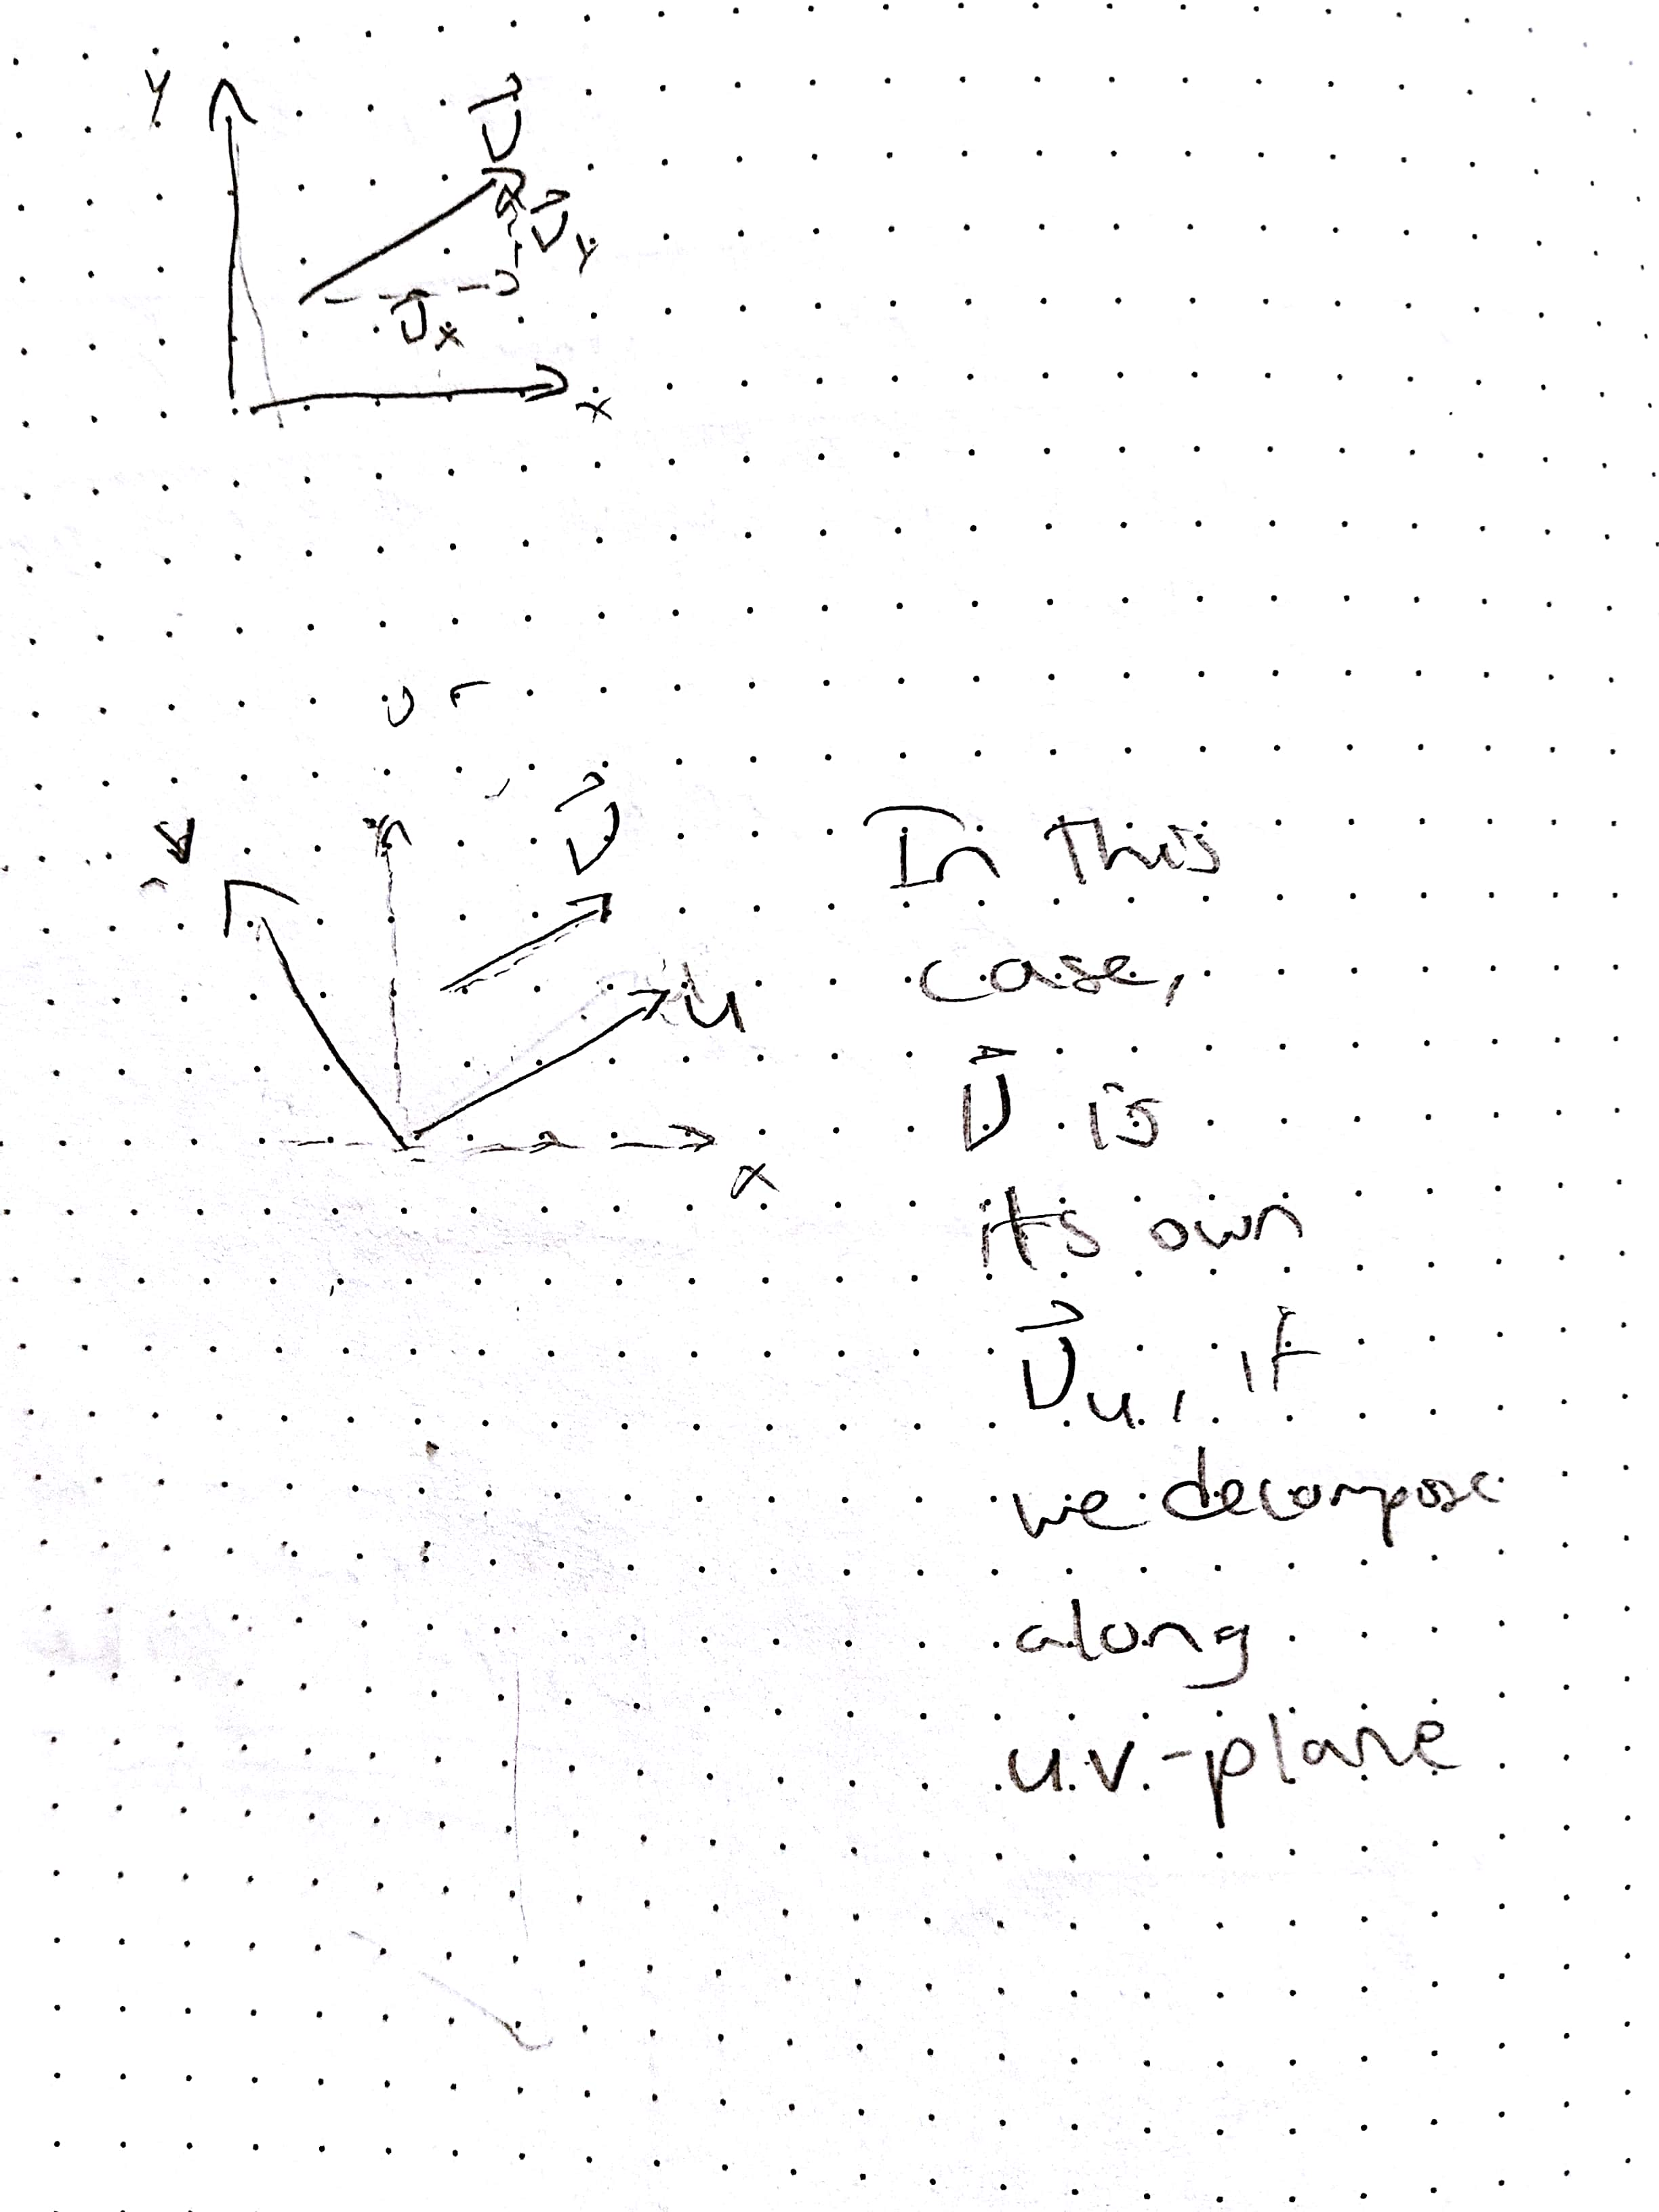
\includegraphics[width=.6\textwidth]{Vectors1.jpg}
    \caption{This image represents how you can decide whatever plane you wish to decompose the vector along. It's important to recognize that the uv-plane can be any arbitrary plane.}
\end{figure}
\\
\\
Now suppose I have some arbitrary vector that I know the magnitude of and direction of. But, consider I only know the direction is 30 degrees north of the positive x axis. This means that my vector should have a 30 degree angle with the x axis and it should point diagonally up-right. So, we have a vector pointing in this direction. Now, if you recall from trigonometry, we can decompose this vector so that we have an x and y component. With a 30 degree angle with the x axis, our x component is like the base of the triangle, or $\text{val}*cos(\ang{30})$. Then our y component is $\text{val}*sin(\ang{30})$. Then, we can represent a vector as its x and y components, as mentioned at the end of the first paragraph: $\vec{V} = <V cos(\theta), V sin(\theta)>$. You may see another notation: $\vec{V} = V cos(\theta) \hat{i} + V sin(\theta) \hat{j}$.\\

\pagebreak

\section{Week 1: Charges and Fields}

If you wish to just learn the equations and general concepts, I'd recommend just the first page of this study guide, since it provides that. If you wish for important concepts that will aid you in thinking, then the Week by Week pages will be useful. I should have a section on vectors if that is a concept you wish to review \\
\\
Primarily, let us quickly discuss the importance of understanding the concept of an electric field. While Coulomb's Law is also very important, an important concept that arises from this class is the concept of fields. As Ghosh said, if previously there was no charge, but suddenly there is, there is suddenly a changing of the space around it. When I say the space changes, I mean that there is a field that other charged particles in the space will feel effects from. So, when we talk about the Coulomb field, we talk about the field due to a charged particle. And just like the gravitational field, electric fields due to singular charges are radial.\\
\\
\textit{Interesting question: If I have 1 charge then suddenly introduce another charge a light year away, would the effect of the distant charge be instantaneous or take time? If it takes time, how long should it take?}\footnote{Electric fields are essentially a result of travelling photons, so we should expect it to take 1 year for our charge to experience the effect of the distant charge}\\
\\
Recall that we learned what an electric field is $\vec{E}$ and Coulombs Law, $\vec{F}_{\text{Coulomb}} = \int \vec{E} dq$. This notation is simply restating the idea of the superposition principle. In fact, we can describe $\vec{E} = \frac{1}{4\pi\epsilon} \int \frac{dq}{|r|^2} \hat{r}$. When we say  $\vec{E} = \frac{1}{4\pi\epsilon} \int \frac{dq}{|r|^2}\hat{r}$, we are saying that what is the net electric field at this point due to all charges. However, in order for the integral to be practical, you should generalize the form. This is quite useful for more convoluted problems. However, when you deal with physical point charges, it's more useful to utilize the general principle (superposition): $\vec{E}_{\text{net}} = \Sigma \vec{E}_i$. This is why you shouldn't ever need to use an integral to deal with problems like Ghosh's example: 4 charges are placed at the edges of a box, and find the force on the charge at the bottom left corner (Which can either be envisioned as the force on that charge due to each of the other charges in the box or the net electric field due to the other charges in the box times the charge you care about).\\
\begin{figure}[ht]
\center
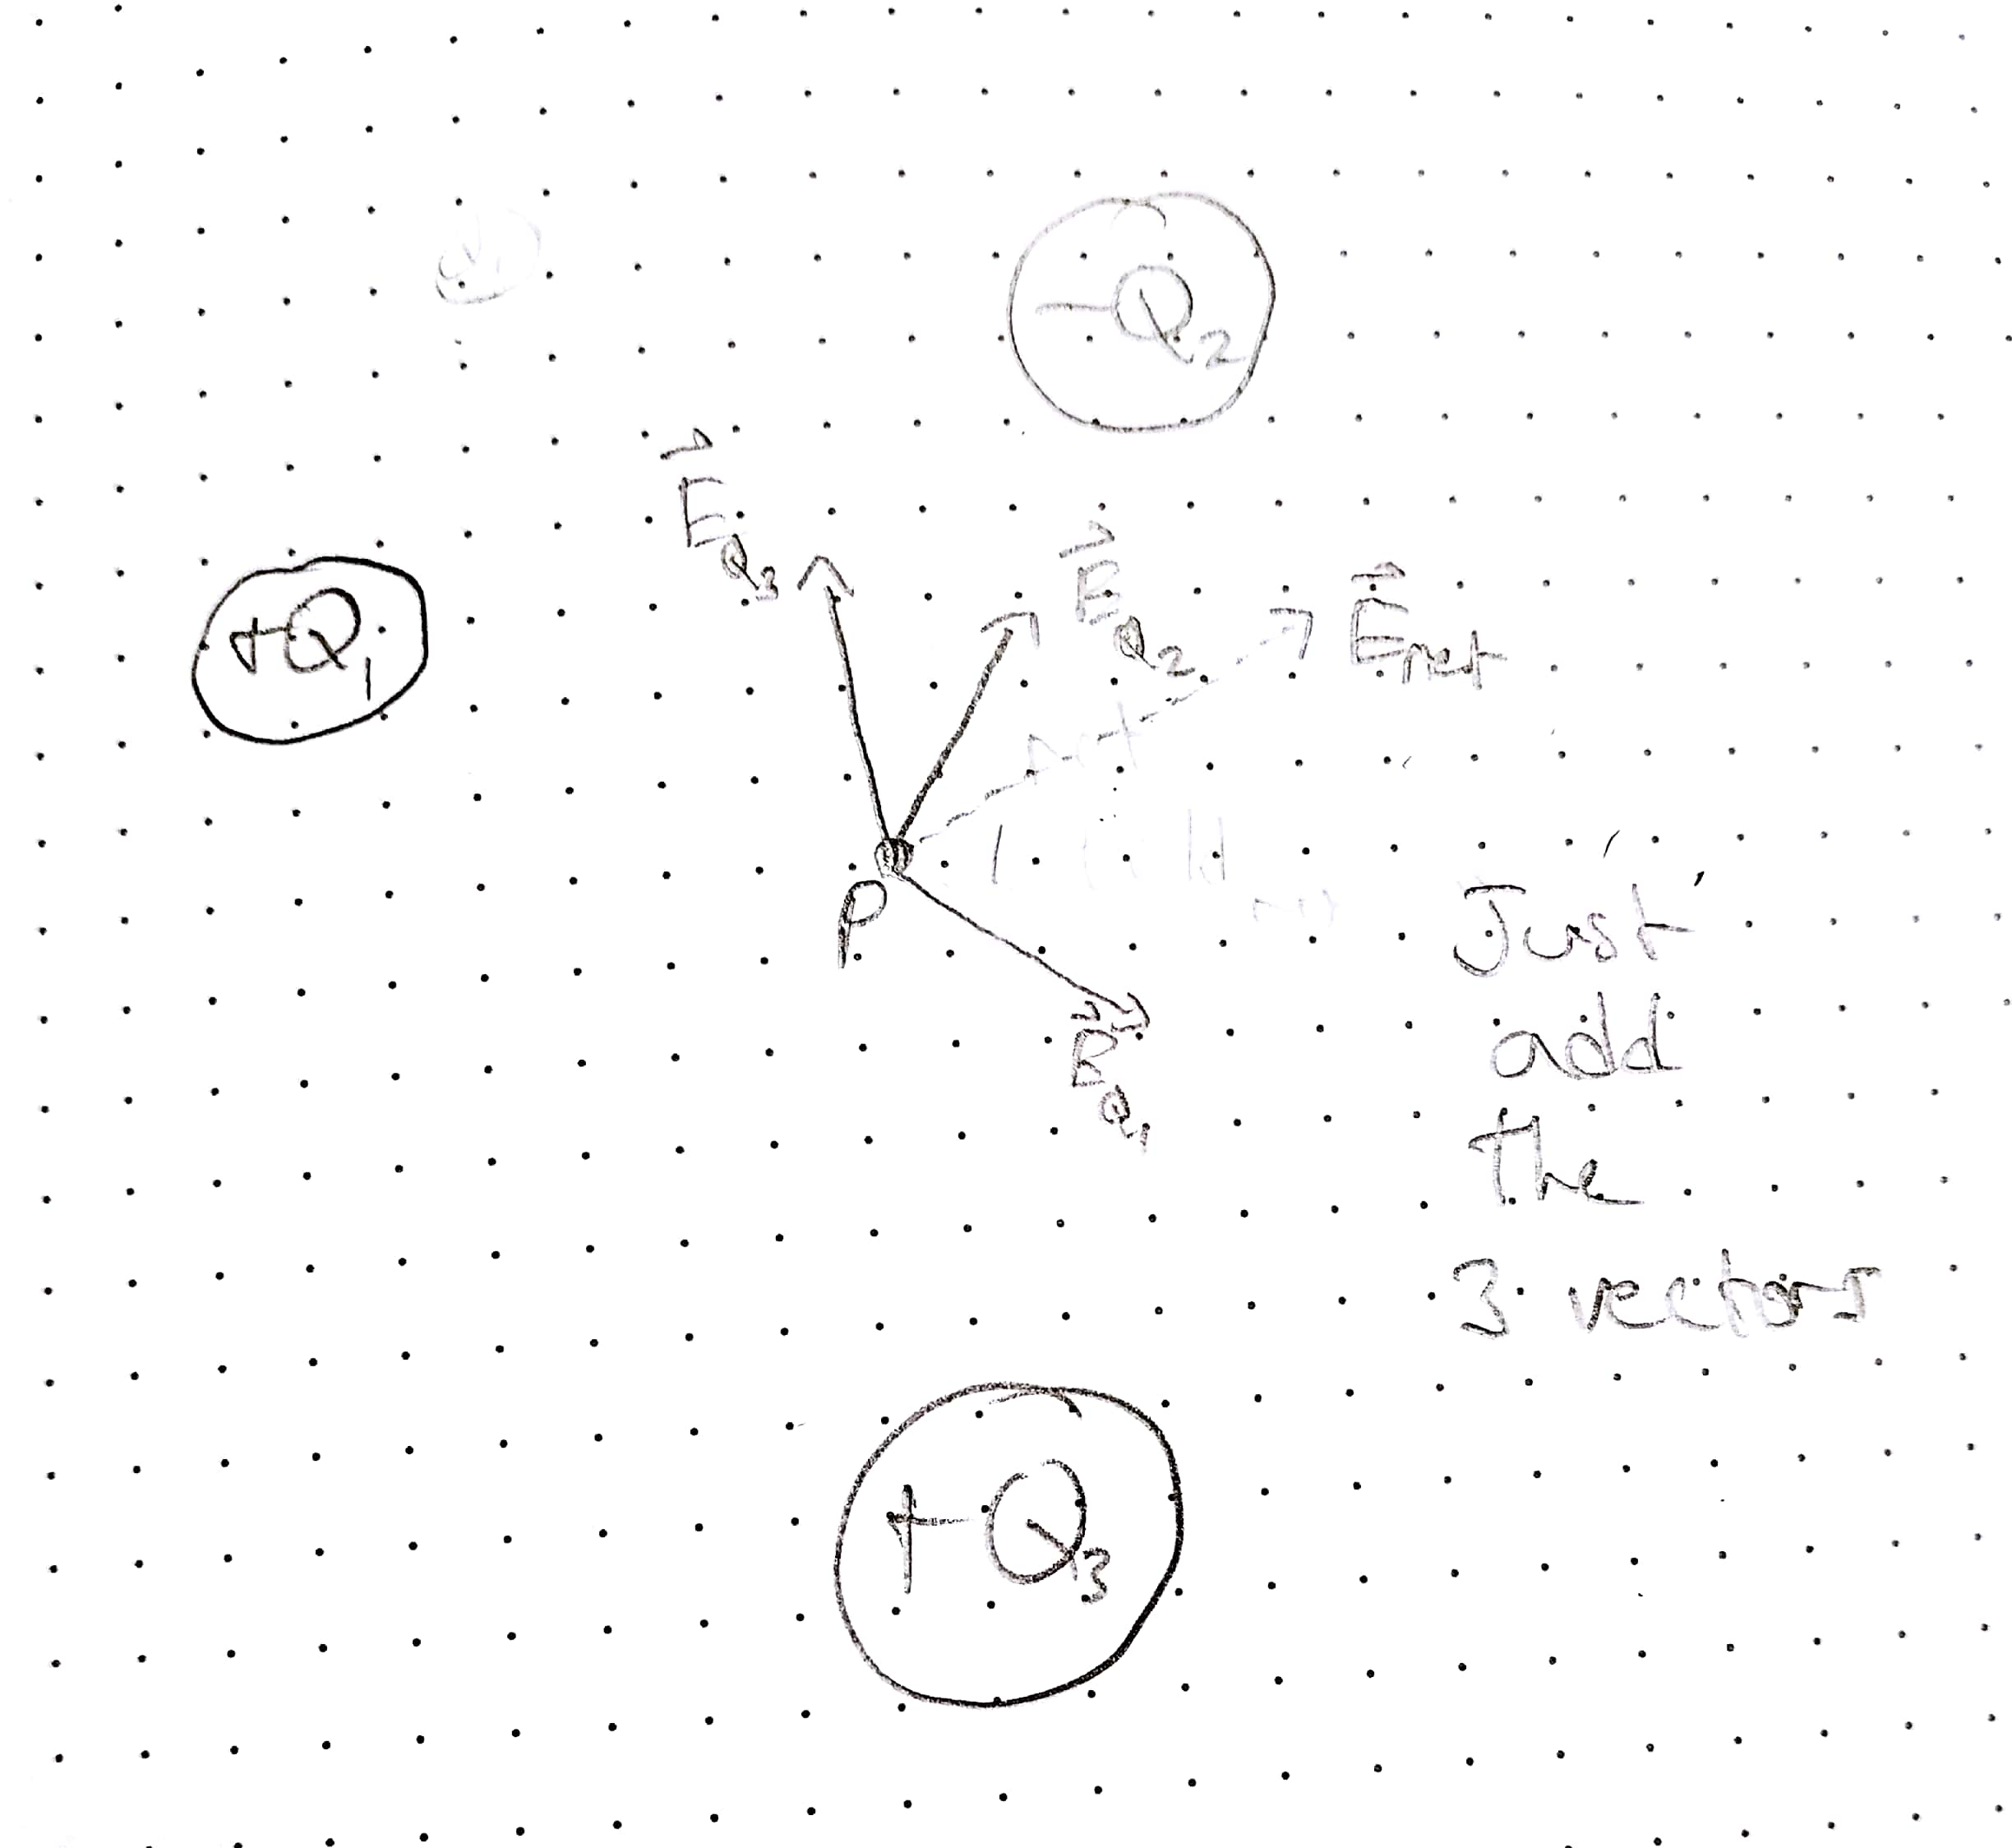
\includegraphics[width=.4\textwidth]{Vectors2.jpg}
\caption{This image represents the idea of superposition. As you can see, the electric field at any point can be represented by the sum of the electric field of every individual electric field at that point (in this case, the sum of electric fields due to individual charges).}
\end{figure}\\
\\
\subsection{Extra Mini Subsection: Dipoles}
Another very important concept in physics is the concept of a dipole. Why is this important? Well, as you'll later learn, many induced charge distributions in materials can be generalized to be a dipole, which tremendously simplifies the problem. In physics, we aim to turn something convoluted into something very simple and beautiful. Now, for a dipole, the general question is, how do I determine the electric field of a dipole. What's even more interesting is that the net charge of a dipole is 0 Coulombs, since there is a positive and negative charge contained in a dipole. However, even still, there should still be a net electric field. To calculate this, we apply the superposition principle again. Calculate the electric field due to one charge and add it to the electric field due to the other charge. For the purposes of this class, we only should be able to determine the electric field along the dipole's axis and the electric field along the perpendicular axis stemming from its midpoint.\\
\begin{figure}[ht]
\center
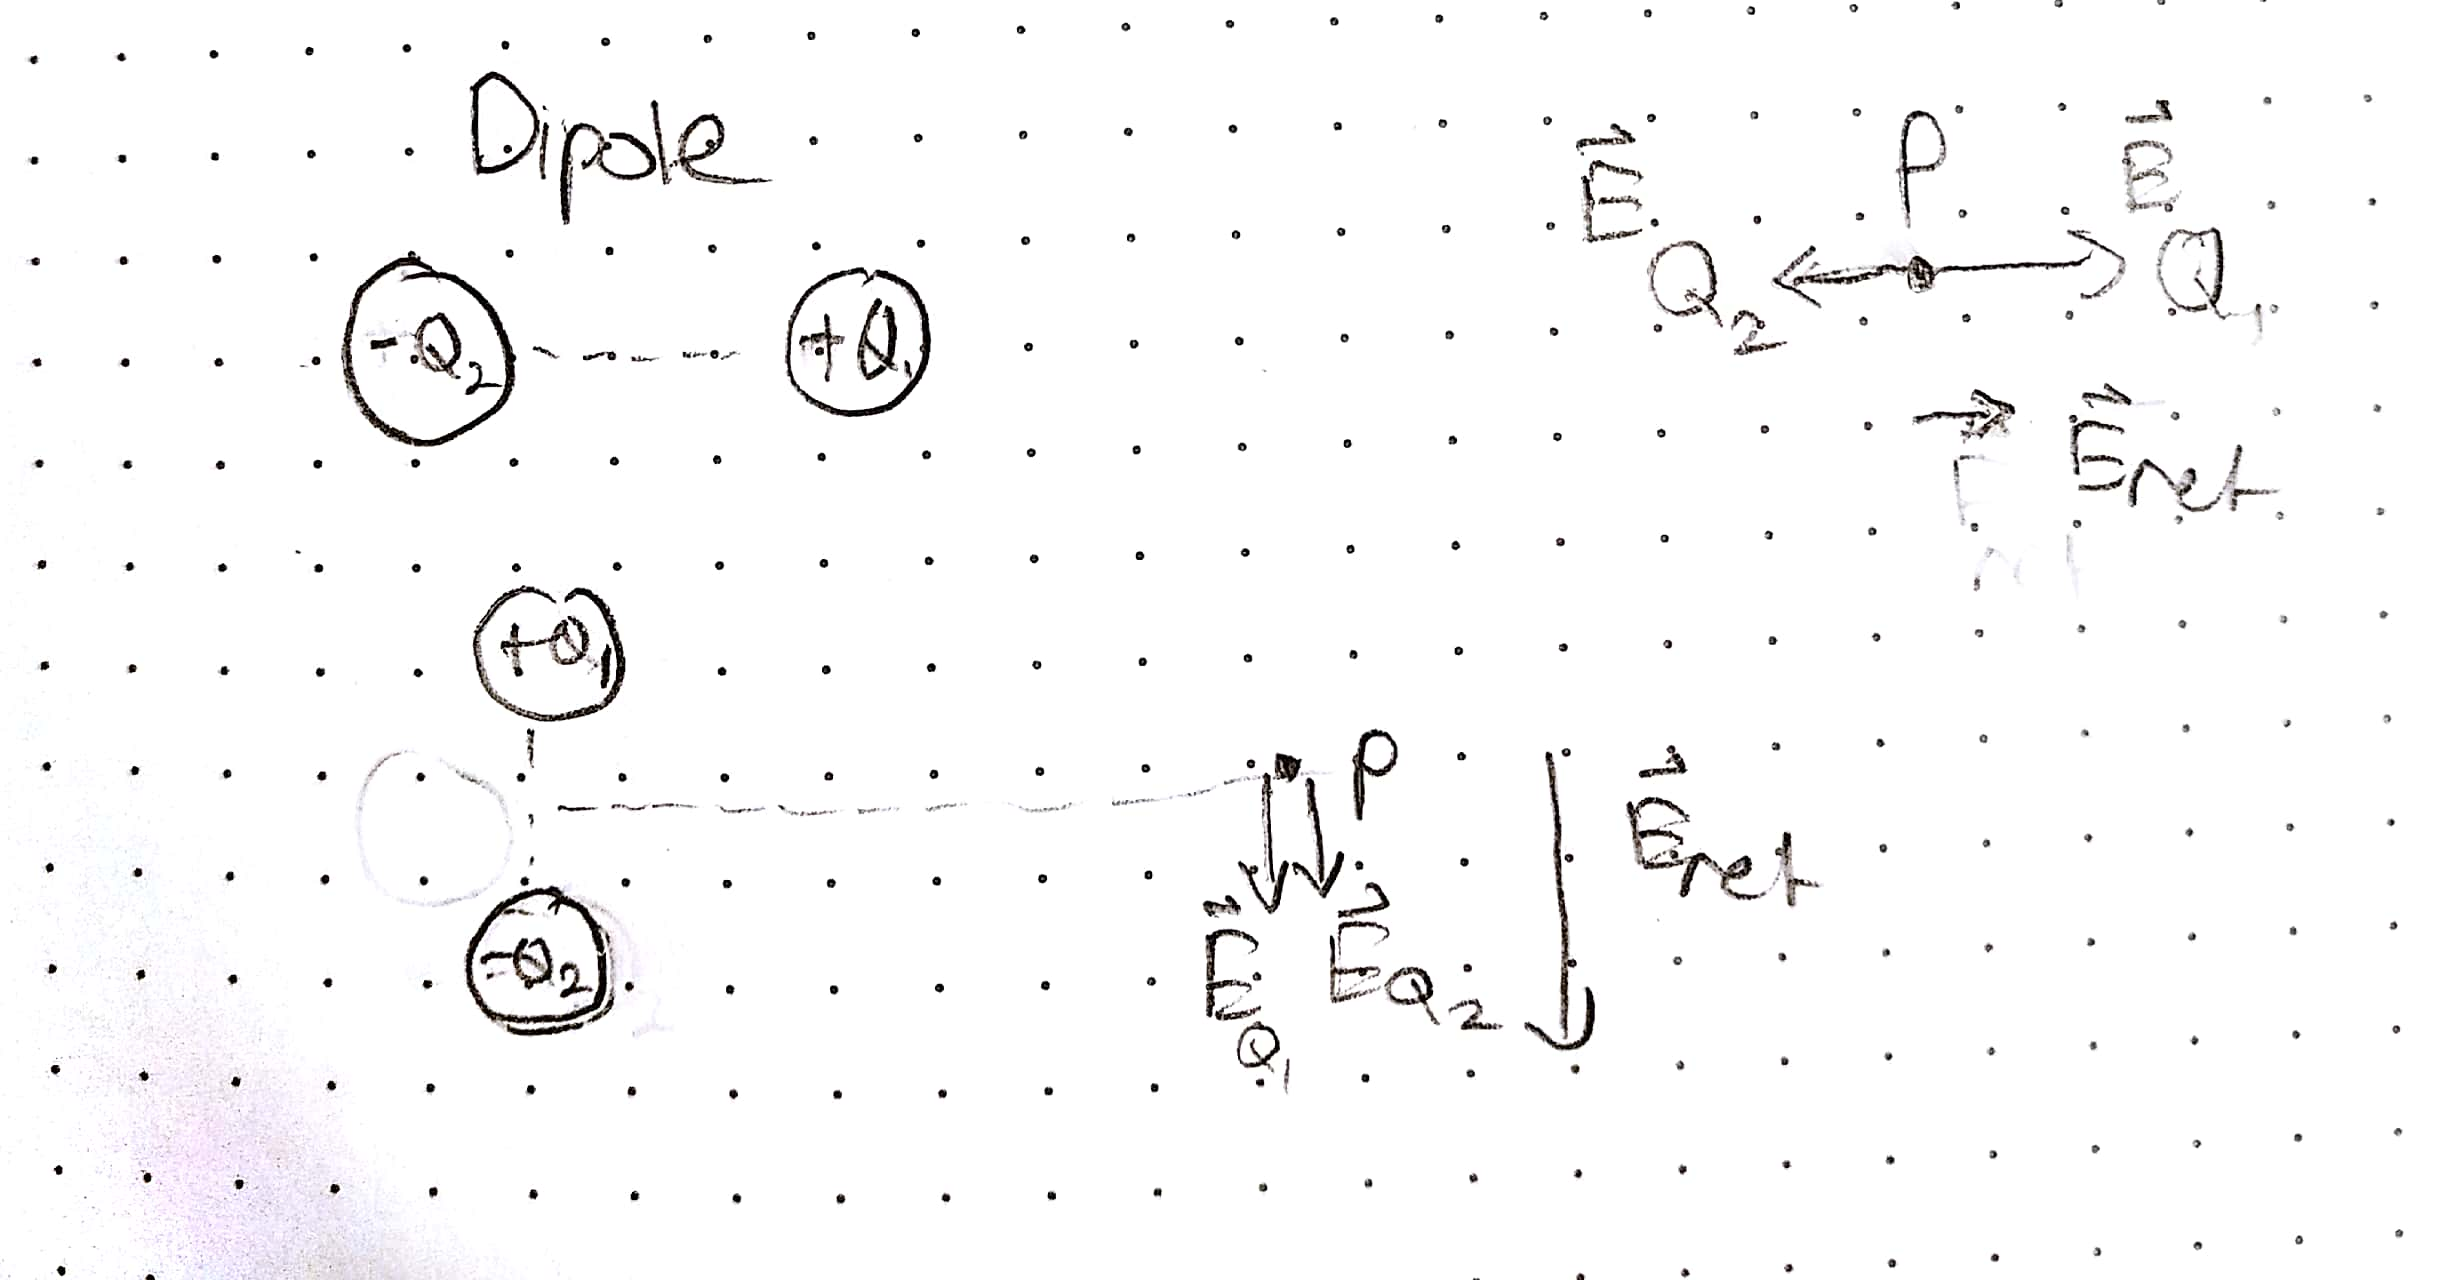
\includegraphics[width=.4\textwidth]{images/Week1pic2.jpg}
\caption{This image demonstrates the general idea you should have when deriving the electric field due to a dipole.}
\end{figure}\\
\\
So, let us proceed by the derivation. Call our distance between the two poles of the dipole to be "d" and the absolute value of the charge of each pole to be "Q". We also want to center our origin to be the center of the dipole, and r is my distance from the center to the point P (Let $r >> d$). Lastly, I am also calculating the electric field along the positive x axis as per the image above. For this study guide, I will only be deriving the along axis electric field. Let the perpendicular problem be something for you to think about or do on your own time. Proceeding, we can describe the electric field: 
\begin{align}
\vec{E}_{Q_1} =& \frac{1}{4\pi\epsilon}\frac{Q}{(r-\frac{d}{2})^2}\hat{x}\\
\vec{E}_{Q_2} =& \frac{1}{4\pi\epsilon}\frac{-Q}{(r+\frac{d}{2})^2}\hat{x}
\end{align}\\
\\
Now, we apply the superposition principle:\\
\begin{align}
\vec{E}_{\text{net}} =& \frac{1}{4\pi\epsilon}\frac{Q}{(r-\frac{d}{2})^2}\hat{x} + \frac{1}{4\pi\epsilon}\frac{-Q}{(r+\frac{d}{2})^2}\hat{x}\\
=& \frac{1}{r^2}(\frac{1}{4\pi\epsilon}\frac{Q}{(1-\frac{d}{2r})^2} + \frac{1}{4\pi\epsilon}\frac{-Q}{(1+\frac{d}{2r})^2})\hat{x}
\end{align}
\\
Why did I pull out an $r^2$ from the denominator? Since my $r >> d$, I know that $\frac{d}{2r} << 1$. So, I can apply the Binomial Expansion. Proceeding, we have:
\begin{align}
\vec{E}_{\text{net}} =& \frac{1}{4\pi\epsilon}\frac{1}{r^2}((Q)(1-\frac{d}{2r})^{-2} + (-Q)(1+\frac{d}{2r})^{-2})\hat{x}\\
=& \frac{1}{4\pi\epsilon}\frac{1}{r^2}((Q)(1+\frac{d}{r}) + (-Q)(1-\frac{d}{r}))\hat{x}\\
=& \frac{1}{4\pi\epsilon}\frac{1}{r^2}(2Q(\frac{d}{r}))\hat{x}\\
=& \frac{1}{4\pi\epsilon}\frac{2Qd}{r^3}\hat{x}
\end{align}\\ \
Recall that this applies to the situation described above. We can generalize this idea by creating a dipole moment vector, defined $\vec{\rho} = Q\vec{d}$, where $\vec{d}$ points from the negative pole to the positive pole of the dipole. This pole direction is the direction of the electric field along its axis around the dipole (Where the electric field between the poles is simply from the positive end to the negative end (opposite direction)). Then our electric field along the axis is condensed to: $$\frac{1}{4\pi\epsilon}\frac{2\vec{\rho}}{r^3}$$\\
\\
Now I want to go back to discussing the mathematical applications of integrals to physics. As was previously discussed, we can represent our electric field as $$\vec{E} = \frac{1}{4\pi\epsilon}\int \frac{dq}{|r|^2}\hat{r}$$The idea behind this description of the electric field is that I want to sum up all the effects of every infinitesimal small piece of charge dq. However, you cannot simply integrate on $dq$ because every $dq$ may have a different position, leading to a dependence on the $r$. In many cases, you can represent $dq$ by $dq = \rho *dV$. $\rho$ would be the charge density as $Q/V$, or charge per volume. However, depending on the symmetry, you can have a different representation for that charge distribution. For example, in a thin rod of charge $Q$ and length $L$, you can utilize the charge distribution in terms of its length (since this rod is thin and uniform and symmetric), $\rho = Q/L$. By understanding this, you can apply this to many problems. One example I will cover is the electric field due to an infinite plate of charge of uniform charge density $\rho$. Note that just because it has a fixed density does not mean that it will have infinite charge because $\rho * \infty$ makes no physical sense (we are doing physics, after all. So infinity is purely a mathematical tool). Thus, let me describe the electric field due to each individual charge at a distance $d$ from the plate: $$\vec{E} = \frac{1}{4\pi\epsilon}\int_{-\infty}^{\infty}\int_{-\infty}^{\infty}\frac{\rho}{|r^2|}\hat{r}dA$$This expression is a tad too complicated for our purposes, since it involves understanding of the double integral. However, we can apply an interesting symmetry trick. A plane of charge is simply an infinite amount of infinite rods on top of each other. So, we can apply our expression for the infinite rod here and integrate along only one direction. Let us choose our rods to be lined up so that they line up along the z axis:
%%%%%% INSERT FIGURE HERE %%%%%%
\\
Our expression for the electric field due to an infinite rod is $$\vec{E}_{inf rod} = \frac{1}{4\pi\epsilon}\frac{2\rho}{r}\hat{r}$$Recall that $\rho$ is the same as $\frac{dq}{dA}$. So we still need to integrate along the z direction. We can apply another interesting thing about symmetry. Since the rods are infinite, we can imagine each rod as a point charge having the electric field of the rod, each charge placed along the midpoint. Then, our $r$ is very simple: $r = \sqrt{y^2 + d^2}$, where there is no $x$ dependence. Finally, let us rewrite our expression: $$\vec{E} = \frac{1}{4\pi\epsilon}\int_{-\infty}^{\infty} \frac{2\rho}{\sqrt{y^2 + d^2}}\hat{r} dy$$We also know that our $\hat{r} = \frac{\vec{r}}{|\vec{r}|} = \frac{1}{\sqrt{y^2 + d^2}}<d,\ y>$. However, again, because of symmetry, we have that our $y$ components should cancel out since the plane is symmetric along positive and negative $y$ axis. So, we only care about the $z$ component: $\vec{z} = \frac{d}{\sqrt{y^2 + d^2}}\hat{z}$. Let us once again rewrite our integral: $$\vec{E} = \frac{1}{4\pi\epsilon}\int_{-\infty}^{\infty} \frac{2\rho d}{y^2 + d^2} dy$$You can then use trigonemtric substitution. As a result of some calculations, the expression condenses to: $$\big|_{-\pi/2}^{\pi/2} 2\rho \theta = \frac{\rho}{2\epsilon}$$

\pagebreak

\section{Week 2}

\pagebreak

\section{Week 3}

\pagebreak

\section{Week 4}

\pagebreak

\section{Week 5}

\pagebreak

\section{Week 6}

\pagebreak

\section{Maxwell's Equations}
This section goes in depth in explaining the implications and intuitions for understanding and using Maxwell's Equations. First, I will write down the 4 equations governing electric and magnetic fields:
\begin{align*}
    \oiint_{\partial \Omega} \VF{E} \cdot \VF{n} \dif S
    &= \frac{1}{\epsilon}\iiint_{\Omega} \rho \dif V\\
    \oiint_{\partial \Omega} \VF{B} \cdot \VF{n} \dif S
    &= 0\\
    \oint_{\partial \Sigma} \VF{E} \cdot \dif \VF{s}
    &= -\frac{\dif}{\dif t}\iint_\Sigma \VF{B} \cdot \dif S\\
    \oint_{\partial \Sigma} \VF{B} \cdot \dif \VF{s}
    &= \iint_\Sigma \VF{J} \cdot \dif \VF{S} + \frac{\dif}{\dif t}\iint_\Sigma \VF{E} \cdot \dif \VF{S}
\end{align*}\\
\subsection{Gauss' Law for Electric Fields}
$$\oiint_{\partial \Omega} \VF{E} \cdot \VF{n} \dif S = \frac{1}{\epsilon}\iiint_{\Omega} \rho \dif V$$\\
\\
When we learn physics, we don't aim to just learn to utilize and memorize the equations. Rather, by understanding intuitively how the concepts are incorporated and how the different operators in the equation work together, you can understand exactly what is being modeled, which also allows you to be able to construct models for more situations.\\
With that being said, let us discuss Gauss' Law. The expression is very complex, but let us dumb it down to a very simple series of explanations. When we see a loop in the double integral, that means a closed surface integral. This is the same as saying: I want to find the flux through the entire surface (all faces). In the expression, we have $$\VF{E} \cdot \VF{n} \dif S$$Know that $\VF{n}$ is the unit vector pointing orthogonal (perpendicular) to the surface. In addition, when we do a dot product $\VF{E} \cdot \VF{n}$, we are saying what is the component of the electric field going perpendicular to the surface. This is multiplied by $\dif S$, or a small piece of area on the surface. So we can visualize this as similar to saying $$\VF{E} \cdot \dif \VF{A}$$which we know to be the definition of the electric flux. Then, the left hand side of Gauss' Law simply says: I want to calculate the entire electric flux through a closed surface. In Gauss' Law, this closed surface is the surface you construct. On the right side, we have $$\frac{1}{\epsilon}\iiint_{\Omega} \rho \dif V$$$\rho$ is our charge density, so by doing a triple integral over our surface, we are saying: What is the charge enclosed by our surface? So the main idea of Gauss' Law is that it relates the electric flux to the charge enclosed. Notice that to utilize Gauss' Law, you should know what the electric field looks like. This is so that you can know how to use ideas like symmetry to get a simple surface where the electric field goes through at a constant angle (hopefully perpendicular) and is constant. If it is constant, then the integral expression can be eliminated if you know the surface area of your surface. \\
\\
\subsection{Gauss' law for Magnetic Fields}
$$\oiint_{\partial \Omega} \VF{B} \cdot \VF{n} \dif S = 0$$\\
\\
Looking at the left side, this is simply the same expression for Gauss' Law for electric fields except replaced with magnetic flux. However, notice how the right hand side is 0. When we think about magnetic fields, we will always have loops. After all, unlike electric fields, magnetic fields always have a north and south pole, so the magnetic field cannot go off indefinitely without ever returning. As a result, when we talk about the closed surface integral, or the flux through the entire surface, we include both the magnetic field going out and the magnetic field coming back. These always cancel out (unless there are magnetic monopoles\footnote{Magnetic Monopoles are an active field of research. In fact, this version of Gauss' Law indicates that if there were monopoles, we would have a non-zero magnetic flux. There is no evidence to suggest that magnetic monopoles cannot exist.}), which leads to the 0.

\end{document}